% This is samplepaper.tex, a sample chapter demonstrating the
% LLNCS macro package for Springer Computer Science proceedings;
% Version 2.20 of 2017/10/04
%
\documentclass[runningheads]{llncs}
%
\usepackage{graphicx}
% Used for displaying a sample figure. If possible, figure files should
% be included in EPS format.
%
% If you use the hyperref package, please uncomment the following line
% to display URLs in blue roman font according to Springer's eBook style:
% \renewcommand\UrlFont{\color{blue}\rmfamily}

\usepackage{times}
\usepackage{graphicx}
\usepackage{latexsym}
\usepackage{amsmath}
\usepackage{algorithm}
\usepackage{algorithmicx}
\usepackage{amsfonts}
\usepackage{amssymb}
\usepackage{bm}
\usepackage{multirow}
\usepackage{threeparttable}
\usepackage{multicol}

\begin{document}
	%
	\title{Synthesis of Registered Multimodal
		Medical Images with Lesions}
	%
	%\titlerunning{Abbreviated paper title}
	% If the paper title is too long for the running head, you can set
	% an abbreviated paper title here
	%\inst{1}
	\author{ Yili Qu \and Wanqi Su \and Chufu Deng \and Ying Wang \\
		\and Yutong Lu \and Zhiguang Chen \and Nong Xiao}
	%
	\authorrunning{Yili, Wanqi et al.}
	% First names are abbreviated in the running head.
	% If there are more than two authors, 'et al.' is used.
	%
	\institute{Sun Yat-sen University,	China,\\
		\email{quyli,suwq7,chufd3@mail2.sysu.edu.cn}}
	%
	\maketitle              % typeset the header of the contribution
	%
	\begin{abstract}
		In a large number of data-driven medical image intelligent processing tasks, the collection and annotation of medical image data is very difficult, especially registered multimodal medical image data. Synthetic medical image data can alleviate the problem of insufficient data well. In this paper, based on the unsupervised conditional GAN model, we achieve the synthesis of registered multimodal medical images from a random normal distribution matrix, and the corresponding lesion information can be efficiently generated based on the freely selected lesion label. We conduct a number of validation experiments on multiple datasets to verify that our synthetic images can be used as pre-trained data or enhanced data in medical image intelligent processing tasks, and they can greatly improve the generalization ability of the model.
		
		\keywords{Image Synthesis \and  Multimodal \and Medical Images \and  Lesions.}
	\end{abstract}
	%
	%
	%
	\section{Introduction}
	In recent years, intelligent medical image processing has become one of the most influential fields in the application of deep learning. Medical images is the images of biological tissue used in medical treatment and obtaine different modalities using different imaging methods . The common modalities include magnetic resonance imaging (MRI), CT, X-ray, etc. Some modalities are divided into different submodalities according to different settings during imaging, such as MRI including T1, T2, T1c and Flair.
	More and more medical images research based on deep learning is expected to obtain a large number of medical images data. However, the collection and annotation of medical image data is very difficult, especially for the registration of multi-mode data. With the development of image synthesis technology, it is possible to synthesize high-quality medical images. This is a good way to alleviate the scarcity of medical images data.
	However, medical images contain complex physiological structure information, and the usual way of synthesis is likely to produce unreasonable structure or contour. On the other hand, the researchers expect multimodal medical images to provide more information for diagnosis. It is also a challenge to ensure the registration of composite image when multimodal image is synthesized.
	Most importantly, the greatest value of medical images is the lesions information. The lesions information in medical images is an important basis for doctors to make diagnosis, s well as an important basis for reasoning and diagnosis of intelligent medical image processing model. Therefore, another big challenge in synthesizing medical images is to control the synthesis of lesions and generate corresponding lesion labels.
	
	With the development of GAN-based image synthesis, GAN has gradually been widely used in medical image segmentation\cite{40kamnitsas2017unsupervised}, reconstruction\cite{61fan2018a,65anirudh2018lose}, synthesis \cite{41costa2017towards,4shin2018medical,43iglesias2013is,44shrivastava2017learning}, translation \cite{2zhang2018translating,20nie2017medical,35osokin2017gans,36vannguyen2015crossdomain,40kamnitsas2017unsupervised,136yi2018sharpness-aware,137yang2018low-dose,138WolterinkGenerative} and super resolution \cite{14You2018CT,15lyu2018super-resolution}. 
	Recently, some studies have attempted to alleviate the difficulty of having few samples of medical image data by synthesizing more diverse data, such as the synthesis of brain MRI\cite{4shin2018medical}, the synthesis of retina \cite{41costa2017towards}, and the synthesis of monomorphic medical images of many different parts and modes\cite{96zhang2019skrgan:}. Among them, the brain MRI synthesis \cite{4shin2018medical} GAN synthetic brain images is applied to implement the image through synthetic data enhancements and anonymous, but its input is extracted from real data structure division of the brain, not only need additional training in tabbed and split, you also need to provide segmentation result in another data set, which makes this method is restricted by many factors. In this study, tumor segmentation tags were added at the time of input for the first time to guide the synthesis of lesions. However, there were no additional constraints during the synthesis process, making the synthesis of lesions extremely uncertain. Retinal synthesis studies\cite{41costa2017towards} achieved the random generation of vascular annotation images by variational self-encoder (VAE) \cite{87kingma2014auto-encoding,88rezende2014stochastic}, and then the color retinal images were synthesized with the synthesized vascular annotation images. The latest SkrGAN\cite{96zhang2019skrgan:} made a monomodal image synthesis attempt, and in line with this research idea, Sobel operator was used to extract sketches containing structural information from medical images, and then further synthesizes medical images. However, similar to other studies, the medical images synthesized by SkrGAN did not consider the synthesis of lesion information or the production of corresponding lesion labels, which made most of the synthesized data unavailable.
	
	To solve these problems, we design a multimodal medical image synthesis scheme, which receive a random normal distribution matrix as input to synthesize a set of registered multimodal MRI images with specify lesions. We conducted synthesis experiments on several public datasets, which fully verified the effectiveness of synthetic lesions and the availability of synthetic data. Our main work includes the following aspects:
	\begin{itemize}
		\item Compared with the current best sketch extraction method, we proposed a more concise and clear structural map extraction method, which can directly extract anatomical structure information from medical images without training.
		
		\item We propose a method based on VAE and GAN, which can synthesize any number of more diverse structural feature graphs from multi-dimensional normal distribution random sampling.
		
		\item We propose a method for synthesizing multimodal medical images with lesions by adding lesion labels. The loss provided by the lesion processor constraint the lesion generation according to label, and the loss provided by the modality translation network constraint multimodal images to be registered.
		
		\item We use synthetic data to train the intelligent medical image processing model, indirectly evaluate the performance and quality of synthetic images through the evaluation of the processing capacity of the model .
	\end{itemize}
	
	\section{Method}
	\label{method}
	Our method includes two stages. In first stages, we obtain a structural map generator to generate structural maps from random normal distribution matrix. In second stages, we train a conditional generator with input of structural maps and lesion labels to synthesize MRI images of different modalities according to different conditionals.
	
	In the following chapters, $E_s $, $G_s$, $D_{z} $, $D_{s} $, $D $ and $D_{t}$ are adjusted on VGG11\cite{102simonyan2014very}, $G_m $, $G$, $G_t$ are adjusted on U-net\cite{6zhu2017unpaired}. $E_s$and the discriminators output two results in the last two layers. $G_s$ is a reverse VGG11. $E_s $ and $G_s$ form a group of VAE\cite{88rezende2014stochastic} structures.$G$and $D$ form a group of ACGAN\cite{98odena2016conditional} structures.$G_t$and $D_t $ constitute a group of CycleGAN. In these improved networks, all pooling are changed to the convolution with same stride, and all deconvolution up-sampling of are changed to the nearest neighbor interpolation up-sampling with a convolution. U-net, VGG11 and SSD\cite{109liu2016ssd:} were used for segmentation, classification and detection as the lesion processor $G_l$ .
	\subsection{Structural map extraction and synthesis}
	We call the images that provides basic contour and structure information structural map. Medical images generated directly from random noise by GAN are difficult to generate realistic structural information. Structural maps can provide necessary basic guidance for the synthesis of medical images. However, general structural features such as retinal vascular maps\cite{41costa2017towards} and brain segmentation labels \cite{4shin2018medical}require additional data and training before extracting from the original image. To solve these problems, we design a method for extracting structural maps directly from brain MRI images, which has the advantages of fast operation, no training, and no additional required data. Then, we can train a generator to generate structural maps from random normal distribution matrixes.
	\begin{algorithm}
		\caption{Structural map extraction}
		\label{alg:1}
		\begin{multicols}{2}
			\begin{algorithmic}[1]
				\State Input grayscale image $x$,
				pixel threshold $alpha$ and $beta$ and $gama$,
				gaussian kernel variance $sigma1$ and $sigma2$
				\State $s1 = reduce\_min(sobel(x))$
				\State $s2 = reduce\_max(sobel(x))$
				\State $s1 = gaussian\_blur(s1,sigma1)$
				\State $s2 = gaussian\_blur(s2,sigma1)$
				\State $s1 = mean(s1) - s1$
				\State $s2 = s2 - mean(s2)$
				\State $s1 = ones \times (s1 > alpha)$
				\State $s2 = ones \times (s2 > alpha)$
				\State $s = ones \times ((s1 + s2)> 0)$
				\State $s = gaussian\_blur(s,sigma2)$
				\State $s = ones \times ((s1 + s2)> beta)$
				\State $s = medfilt(s)$
				\State $s = s \times (x > gama)$
			\end{algorithmic}  
		\end{multicols}
	\end{algorithm}
	\subsubsection{Structural map extraction method}
	In traditional digital image processing methods, Roberts operator\cite{145Roberts}, Prewitt operator\cite{146prewitt}, Sobel operator\cite{147Sobel} are excellent edge detection operators. Sobel operators are particularly applicable and are most commonly used to process medical images. Algorithm~\ref{alg:1} describes our feature graph extraction method based on Sobel operator, where  $gaussian\_blur()$ is 3$\times$3 gaussian blur and  $medfilt()$ is 3$\times$3 median filter function.
	\subsubsection{Structural map generation training}
	\begin{algorithm}
		\caption{Mask extraction}
		\label{alg:2}
		\begin{multicols}{2}
			\begin{algorithmic}[1]
				\State Input grayscale image $x$,  pixel threshold $alpha$, expanded pixel width $p$
				\State $m = 1.0 - ones \times (x > alpha)$
				\State $size=[x.width()+p, x.length()+p]$
				\State $m = resize(m, size)$
				\State $m = crop\_padding(m,p)$
				\State $m = medfilt(m)$
			\end{algorithmic}  
		\end{multicols}
	\end{algorithm}
	\begin{figure}
		\centering
		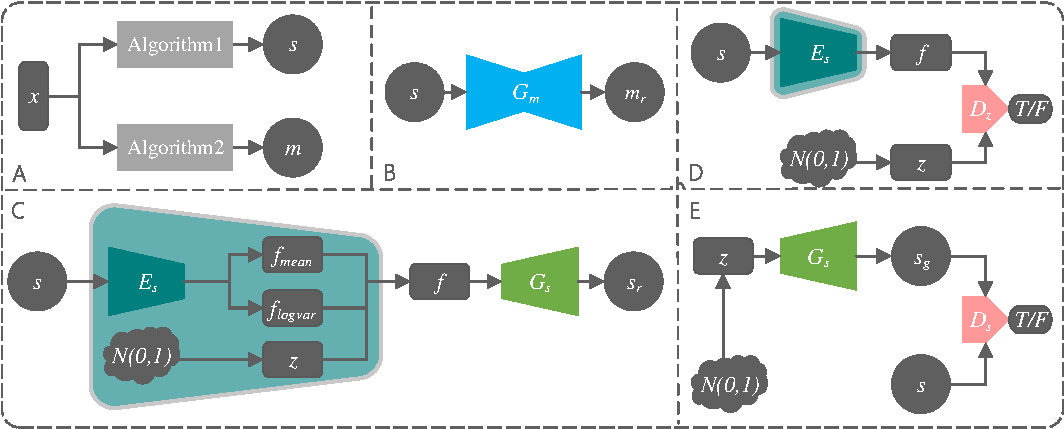
\includegraphics[width=0.98\columnwidth]{figures/feature_train}
		\caption{Structural map generation training. $x$ is an input real image, $s$ is a structural map, $m$ is a mask. $E_s$ is a VAE encoder, which outputs the encode matrixs $f_{mean}$ and $f_{logvar}$. $z$ is a random noise sampling from multidimensional normal distribution $\mathcal{N}(0,1^2)$ and the $f$ is a approximate normal distribution matrix. $G_s$ is a VAE decoder, $s_r$ is a reconstructed structural map, and $s_g$ is a generated random structure feature map. $D_{s}$ and $D_{z}$ are the discriminators. $G_m$ is a mask generator and $m_r$ is a extracted mask. }
		\label{feature_train}
	\end{figure}
	The structural map traing as shown in Fig.~\ref{feature_train}, where $f=f_{mean}+exp(0.5\times f_{logvar})\times z$. Fig.~\ref{generated_f} shows examples of structural maps on BRATS2015. The training losses in Fig.~\ref{feature_train} are as follows, where $\mathbb{E}$ is the expectation operator,$m_r=G_m(s)$,$s_r=G_s(f)$,$s_g=G_s(z)$,$m_g=G_m(s_g)$: 
	\begin{itemize}
		\item{Part B: Mask generation loss}
		\begin{equation}
		\mathcal{L}_{m}(G_m)=\mathbb{E}_{m,s}[\Vert{m-m_r}\Vert_{2}^{2}],
		\end{equation}
		\item{Part C: Structural map reconstruction loss} 
		\begin{equation}
		\mathcal{L}_{r}(E_s,G_s)=\mathbb{E}_{s,f,m}[\Vert{s-s_r}\Vert_{2}^{2}+\Vert{m_r\times s_r}\Vert_{2}^{2}],
		\end{equation}
		\item{Part D: Distribution encoding adversarial loss} 
		\begin{equation}
		\mathcal{L}_{d1}(D_{z})=\mathbb{E}_{s,z}[\Vert{D_{z}(z)-1}\Vert_{2}^{2}+\Vert{D_{z}(f)}\Vert_{2}^{2}].
		\end{equation}
		\begin{equation}
		\mathcal{L}_{g1}(E_s)=\mathbb{E}_{z}[\Vert{D_{z}(f)-1}\Vert_{2}^{2}].	
		\end{equation}
		\item{Part E: Structural map decoding adversarial loss} 
		\begin{equation}
		\mathcal{L}_{d2}(D_{s})=\mathbb{E}_{s,z}[\Vert{D_{s}(s)-1}\Vert_{2}^{2}+\Vert{D_{s}(s_g)}\Vert_{2}^{2}].
		\end{equation}
		\begin{equation}
		\mathcal{L}_{g2}(G_s)=\mathbb{E}_{z}[\Vert{D_{s}(s_g)-1}\Vert_{2}^{2}++\Vert{m_g\times s_g}\Vert_{2}^{2}].	
		\end{equation}
	\end{itemize}
	\begin{figure}[thbp!]
		\centering
		\includegraphics[width=0.85\linewidth]{figures/brats_f}
		\caption{Structural map on BRATS2015.(a) Followed by T1, T2, T1c, Flair four modal of MRI, extracted from Flair mask, extracted from Flair using Sobel operator level to vertical edge detection results and figure, extracted from Flair structure diagram, sign a mask to remove the tumor by splitting the tumor lesion structure information extracted from Flair's structure characteristic figure, tumor segmentation tags binarization mask.(b) Synthesized structural map randomly.(c) Synthesized structural map from sequence sampling on normal distribution.}
		\label{generated_f}
	\end{figure}
	\begin{figure}[thbp!]
		\centering
		\includegraphics[width=0.85\linewidth]{figures/image_f_mask_newf}
		\caption{Medical image and extraction structural map. (a) DRIVE retinal image . (b) Kaggle Chest X-ray. (c) Kaggle Lung CT. (d) TC Lung CT. From left to right are the original image, structural map, mask, and structural map fused noise.}
		\label{image_and_f}
	\end{figure}	
	\subsubsection{Structural map fusion noise}	
	The structural map is a simple binary sparse matrix, and input directly will reduce the diversity and randomness. The equation $s'=s+z'\times(1-m)\times(1-s)$ is used to add random noise to the structural map in the region of organ generation,where, $z'\sim\mathcal{U}(\alpha_1,\alpha_2)$. The default values of $\alpha_1,\alpha_2$ are 0.5 and 0.6 respectively. $m$is a binary mask paired with the structual map $s$. As shown in the Fig.~\ref{image_and_f}, the final fusion structural map $s'$not only retains all the structure information, but also has rich random information. At the same time, it is closer to the expected medical image, which reduces the learning difficulty. 
	\subsection{Multimodal images synthesis}
	\begin{figure}
		\centering
		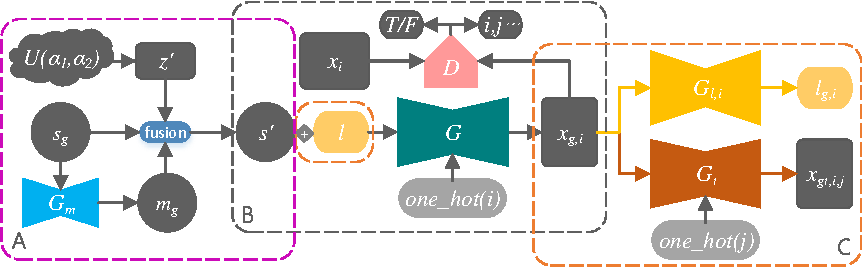
\includegraphics[width=1\columnwidth]{figures/mm_mri_generate_train}
		\caption{Synthesis of multimodal images. Purple box A is the fusion process of structural map and random noise, gray box B is the core process, and yellow box is the optional process. 
			$x_{g,i}$ is the image of modality $i$ generated by generator $G$. 
			$l_{g,i}$ is the lesion label of modality $i$ generated by lesion processor $G_{l,i}$.
			$x_{gt,i,j}$ is the image of modality $j$ translated from modality $i$ by modality translation network $G_t$.
		}
		\label{mm_mri_generate}
	\end{figure}
	As shown in Fig.~\ref{mm_mri_generate}, we get $s_g$ through the trained $G_s$ and fuses the random noise, then concatenate the specified lesion label $l$ according to the need. When selecting a lesion label, the randomly selected label may indicate a lesion that is not in the organ described in the structural map. We used the mask corresponding to the structural map to filter out the labels that the lesion was not within the scope of the organ mask. Then, $G$ accepts the onehot condition matrix $one_hot(i)$ after encoding the fusion input, and then decodes to generate the modality $i$ image $x_{g,i}$. The lesion processor $G_{l,i}$ and the modality translation network $G_t$ train completedly in advance to provide the lesions generation guidance loss and the registration guidance loss for $G$.
	
	The loss items are as follows, where $d(x_{i})$ and $c(x_{i})$ are the true/false discrimination and category discrimination of the discriminator $D(x_i)$, $d(x_{g, i})$ and $c(x_{g,i})$ are the output of $D(x_{g,i})$, and $concat()$ is the concatenate function on feturemap channel. 
	\begin{itemize}
		\item{Adversarial loss}
		\begin{equation}
		\begin{split}
		\mathcal{L}_{d2}(D)=\mathbb{E}_{x,s_g,l}[\sum\limits_{i=0}(\Vert{d(x_i)-1}\Vert_{2}^{2}+\Vert{d(x_{g,i})}\Vert_{2}^{2}+\\
		\Vert{c(x_i)-i}\Vert_{2}^{2}+\Vert{c(x_{g,i})-i}\Vert_{2}^{2})],
		\end{split}
		\end{equation}
		\begin{equation}
		\mathcal{L}_{g}(G)=\mathbb{E}_{s_g,l}[\sum\limits_{i=0}(\Vert{d(x_{g,i})-1}\Vert_{2}^{2}+\Vert{c(x_{g,i})-i}\Vert_{2}^{2})].
		\end{equation}
		\item{Lesion generation guidance loss}
		\begin{equation}
		\mathcal{L}_{les}(G)=\mathbb{E}_{s_g,l}[\sum\limits_{i=0}(\Vert{l-l_{g,i}}\Vert_{2}^{2})].
		\end{equation}
		\item{Rregistration guidance loss}
		\begin{equation}
		\mathcal{L}_{reg}(G)=\mathbb{E}_{s_g,l}[\sum\limits_{j=0}\sum\limits_{i=0,i\neq j}(\Vert{x_{g,i}-x_{gt,j,i}}\Vert_{2}^{2})].
		\end{equation}
	\end{itemize}
	We can also use the structural feature map extracted from the real image and the real medical image for self-supervised pre-training to accelerate the process of antagonistic training. The loss of the pre-training process is as follows:
	\begin{equation}
	\mathcal{L}_{p}(G)=\mathbb{E}_{s,l}[\sum\limits_{i=0}(\Vert{x_{g,i}-x_i}\Vert_{2}^{2}+\Vert{x_{g,i}\times m_i-x_{i}\times m_i}\Vert_{2}^{2})].
	\end{equation}
	In the training of SkrGAN\cite{96zhang2019skrgan:}, real sketch training and self-supervision loss are always adopted, which makes the model too few training samples, insufficient training, easy to over-fit and lack of adaptability to the composite sketch, which will eventually lead to the lack of diversity of the composite image. We used real structure diagrams for self-supervised pre-training and a large number of composite structure diagrams for adversarial training, which can not only accelerate the training process, but also enhance the generalization ability of model. Fig.~\ref{generated_mri} shows examples of images obtained from all stages on BRATS2015.
	\begin{figure}
		\centering
		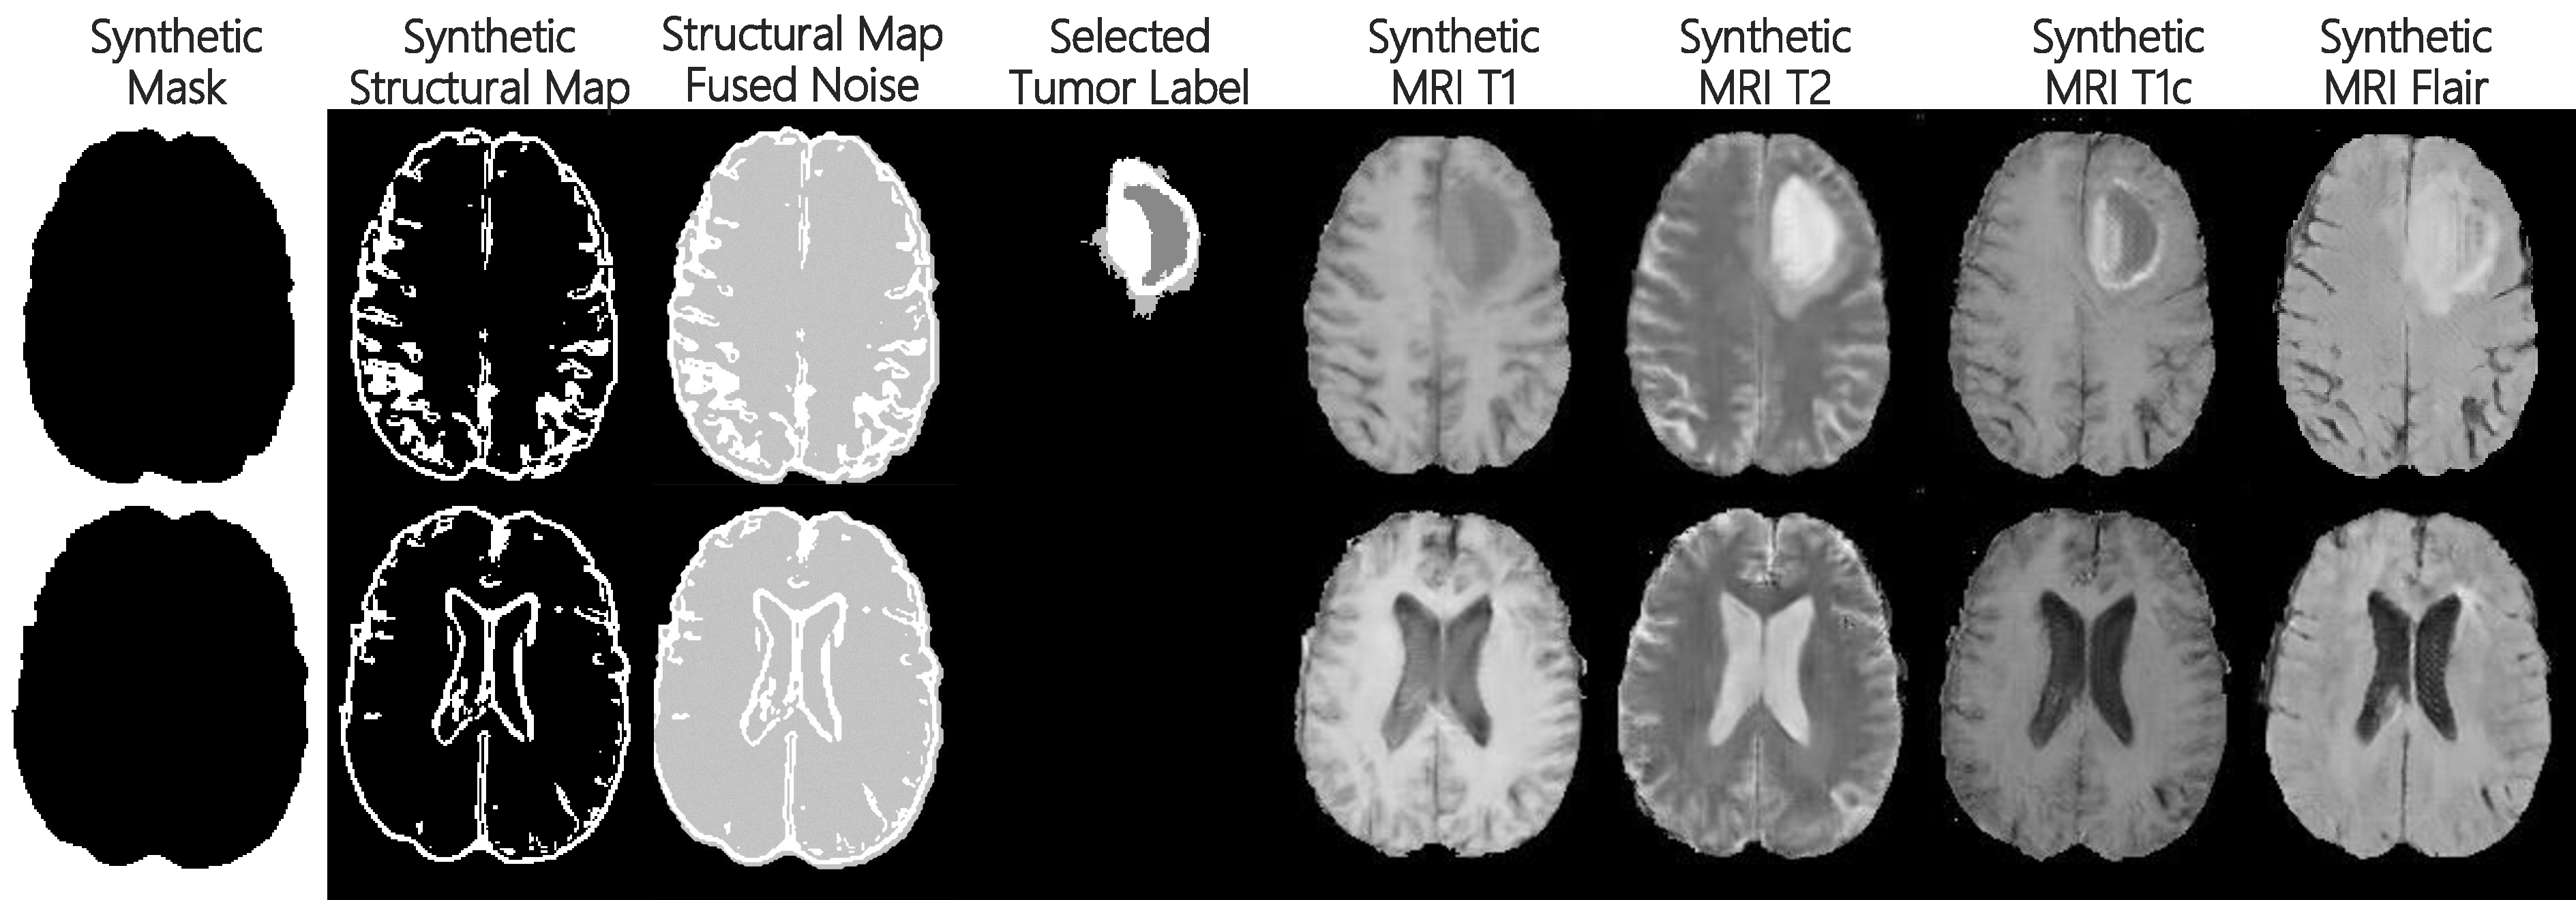
\includegraphics[width=0.6\linewidth]{figures/F_to_MRI}
		\caption{Multimodal images synthesis on BRATS2015.}
		\label{generated_mri}
	\end{figure}
	\subsection{Translation and lesion processing training}
	Before multimodal images synthesis, we perform lesion processing and translation training on real data. The losses of $G_t$,$D_t$ include adversarial loss same as  $G$,$D$ and cycle consistency loss in CycleGAN.
	The losses of $G_{l,i}$ are 
	\begin{equation}
	\label{lesion segmentation loss}
	\mathcal{L}_{seg}(G_{l,i})=\mathbb{E}_{l,x}[\Vert{l_i-G_{l,i}(x_{i})}\Vert_{2}^{2}].
	\end{equation}
	
	\section{Experiments}
	\subsection{Datasets}
	\textbf{BRATS2015\footnote{https://www.smir.ch/BRATS/Start2015}} includes registered T1,T2,T1c,Flair, 274 155$\times$240$\times$240 MRIs per modality wihe tumor segmentation labels. We divide the 3D MRIs to 2D.\textbf{Kaggle Chest X-Ray\footnote{https://www.kaggle.com/paultimothymooney/chest-xray-pneumonia }} includes 5863 positive X-ray grayscale images of viral pneumonia, bacterial pneumonia and normal lungs from 384$\times$127 to 2772$\times$2304.\textbf{Kaggle Lung CT\footnote{https://www.kaggle.com/kmader/finding-lungs-in-ct-data/data/}} includes 267  CT grayscale images of transverse sections from chest to abdomen, with a size of 512$\times$512. \textbf{DRIVE\footnote{http://www.isi.uu.nl/Research/Databases/DRIVE/}} includes 20 565 $\times $584 color fundus retinal photos in both training set and test set and 20 corresponding retinal vascular annotations for training.\textbf{FIRE\footnote{https://projects.ics.forth.gr/cvrl/fire/}} includes 268 2912$\times$2912 color fundus retinal photos.\textbf{TC Lung CT\footnote{https://tianchi.aliyun.com/competition/entrance/231724/information}} includes 1470 512$\times$512 3D CT scans with detection label of 5 kinds of lesions. We only test for pulmonary nodules and using 3-channel image composed of three adjacent slices. All images are normalized and scaled to 512$\times$512.
	
	\subsection{Experiments settings}
	Each experiment was fully trained with more than 100 epochs. The learning rate is 1e-5 with 4 batch size. We use the Adam optimizer with beta1 of 0.5.
	We base our results on the current best quality synthesis achieved in SkrGAN\cite{96zhang2019skrgan:}. We used multi-scale structural similarity (MS-SSIM) and FreshetInception distance (FID)\cite{148karras2017progressive} to assess the performance of synthetic medical images. Dice Score\cite {95dice1945measures} and mean square error (MSE) were used to evaluate the segmentation results. Sensitivity, Accuracy and area under the ROC curve (AUC) were used to evaluate vascular annotation results. Accuracy was used to evaluate the classification results of this study. The Average Precision (AP) was used to evaluate the detection results.The evaluation results in this paper are the average of all the modal results on 2D images, and the results of each experiment are the best results reserved after at least 4 training sessions.
	
	\subsection{Ablation experiments on BRATS2015}
	\begin{table}[thbp!]
		\newcommand{\tabincell}[2]{\begin{tabular}{@{}#1@{}}#2\end{tabular}}
		\caption{Ablation experiments on BRATS2015}
		\label{Ablation Experiment Setting on BRATS2015}
		\centering
		\resizebox{\textwidth}{15mm}{
			\begin{tabular}{c|c|c|c|c|c|l}
				%\toprule
				\hline
				Test		&\tabincell{c}{Input \\structural map} &\tabincell{c}{Fusion\\ noise} &\tabincell{c}{with $\mathcal{L}_{reg}$}   &\tabincell{c}{Input lesion \\label and with $\mathcal{L}_{les}$} &\tabincell{c}{Using mask select\\ lesion label} &MS-SSIM   \\
				%\midrule
				\hline
				\tabincell{l}{A}	&$\times$	&$\times$	&$\times$	&$\times$	&$\times$ &0.504 \\
				\tabincell{l}{B}	&$\surd$	&$\times$	&$\times$	&$\times$    &$\times$ &0.654\\
				\tabincell{l}{C}	&$\surd$	&$\surd$	&$\times$	&$\times$	&$\times$ &0.671\\
				\tabincell{l}{D}	&$\surd$	&$\surd$	&$\surd$	&$\times$	&$\times$ &0.674\\
				\tabincell{l}{E}	&$\surd$	&$\surd$	&$\surd$	&$\surd$	&$\times$ &0.673\\
				\tabincell{l}{F}	&$\surd$	&$\surd$	&$\surd$	&$\surd$	&$\surd$ &0.686\\
				\hline
				%\bottomrule
			\end{tabular}
		}
	\end{table}
	Table~\ref{Ablation Experiment Setting on BRATS2015} shows the setting and results of the ablation experiments of our method.
	Fig~\ref{ablation_and_seg} (a) shows examples of synthetic images generated in ablation experiments. 
	\textbf{A} no contour from structural map, the generated image conforms to the features of MRI, but not to the structural features of the brain. 
	\textbf{B} was poorly trained due to lack of a random sample.
	\textbf{C} registration effect is imprecise, especially the edge details.
	Lesions in \textbf{D} were random and exaggerated, which did not match the input  label. 
	Tumor in \textbf{E} was beyond the contours of the brain. 
	\textbf{F} adopts the our complete scheme with best synthesis quality. It can be seen that all the improvements have improved the authenticity of the synthesized image. However, if the lesion labels are added for lesion generation guidance,  the labels need to be screened.
	\begin{figure}
		\centering
		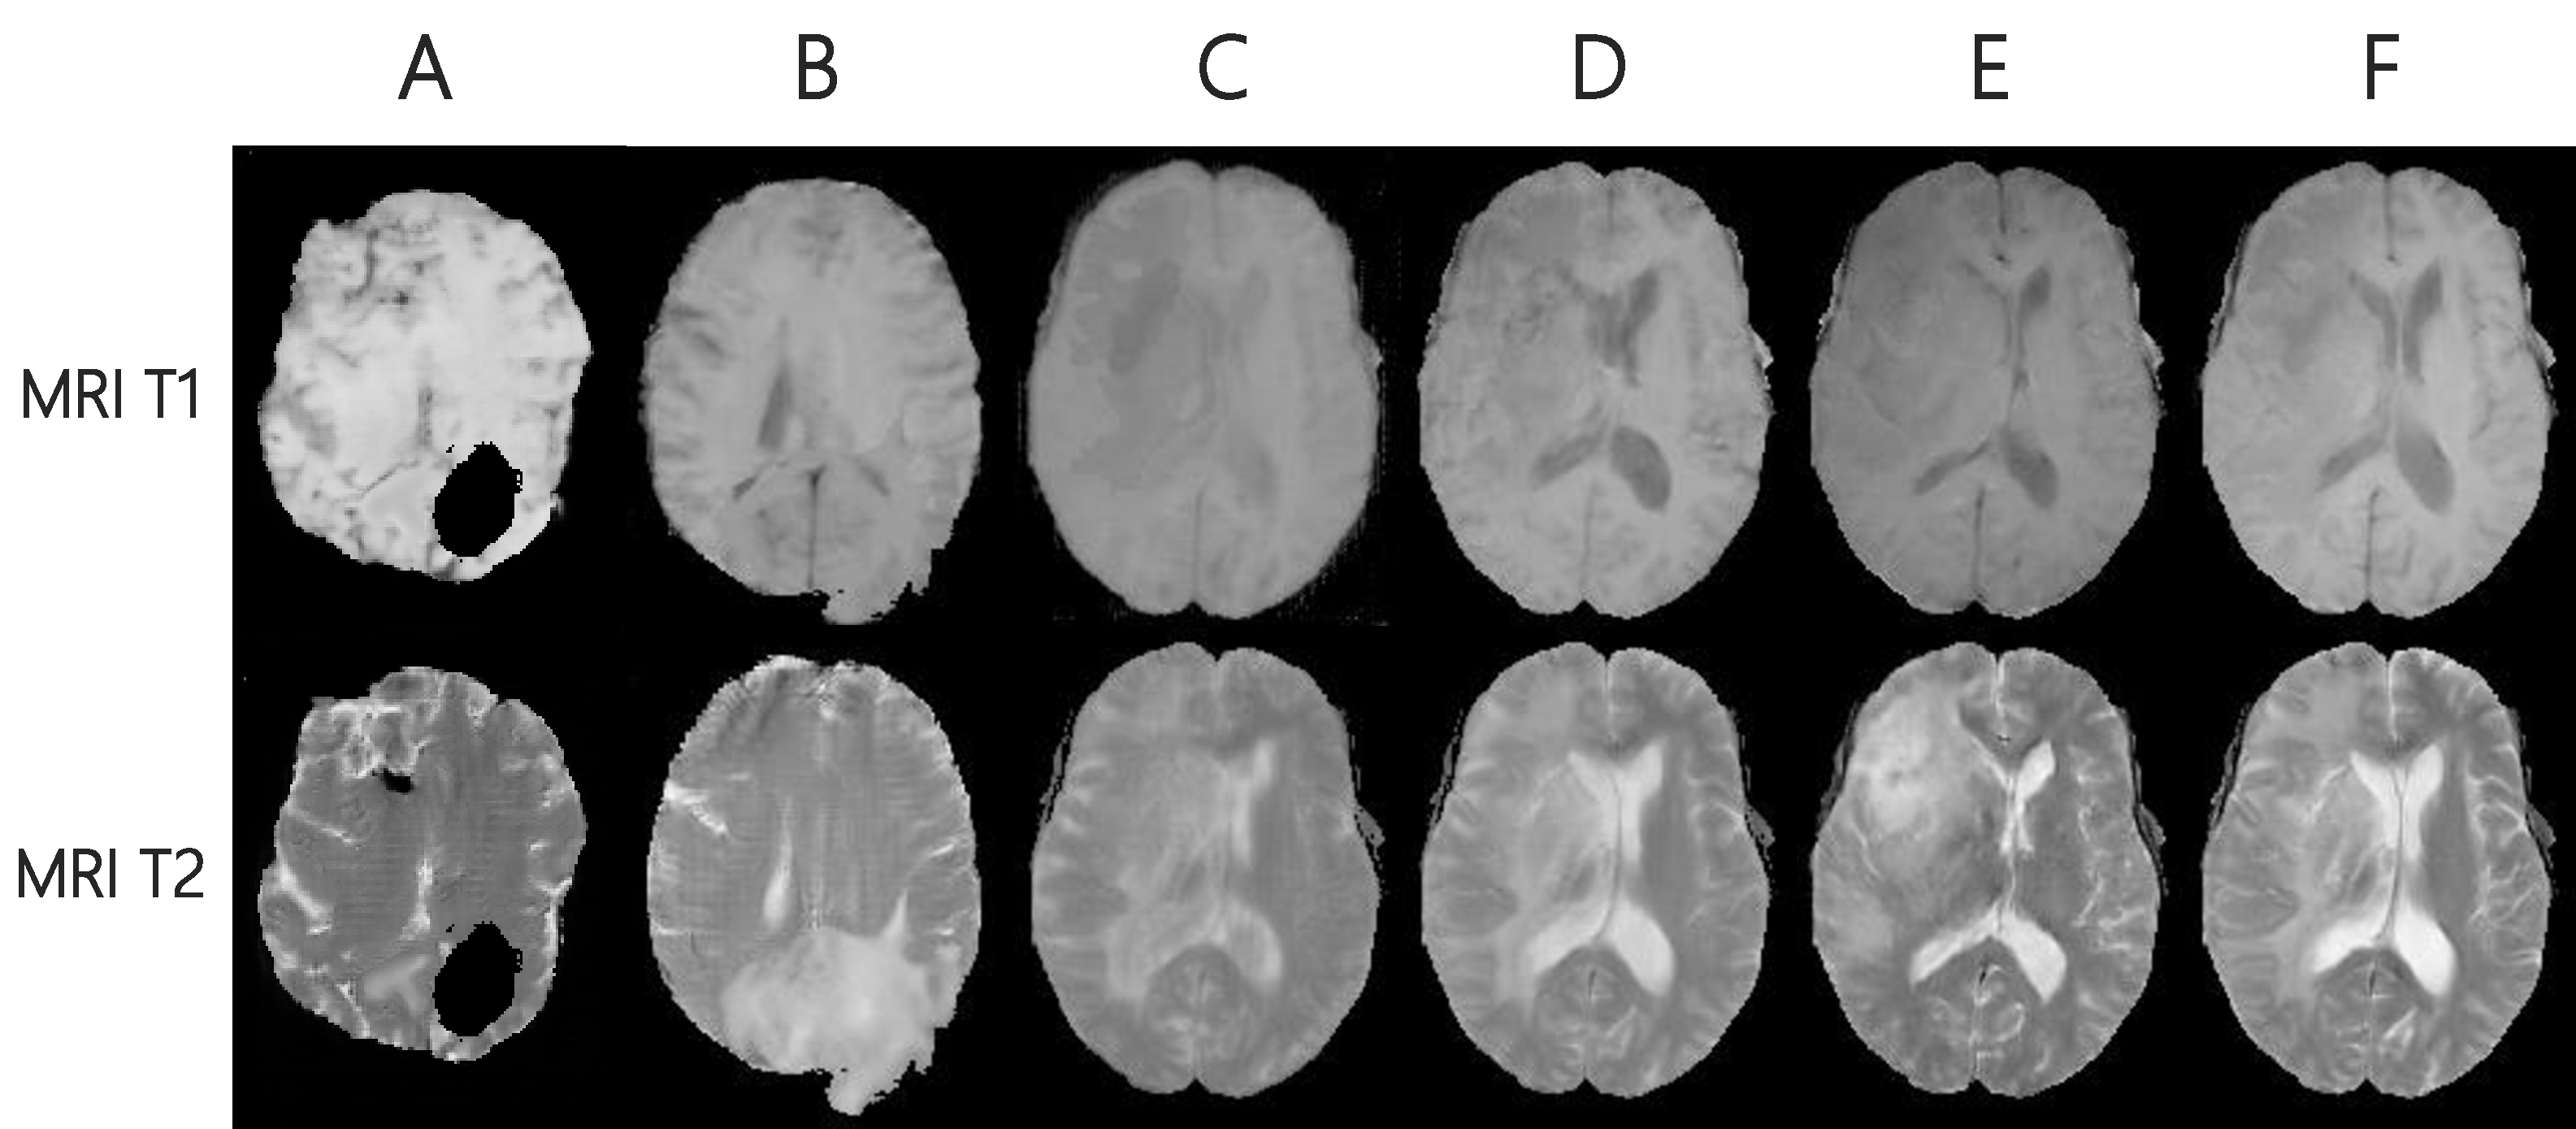
\includegraphics[width=0.85\linewidth]{figures/ablation}
		\caption{(a) Synthetic MRIs of ablation experiments. (b) Segmentation results of synthetic MRI. }
		\label{ablation_and_seg}
	\end{figure}
	\begin{table}
	\begin{center}
		\caption{Lesion generation methods experiments.}
		\label{label_test}
		\begin{tabular}{llccc}
			\hline	
			Trainging Dataset &Test Dataset &MSE   &Dice score \\
			\hline
			real &real 	    &0.027          &0.915 \\							
			real &synthetic	&\textbf{0.043} &\textbf{0.838} \\
			\hline
		\end{tabular}
	\end{center}
\end{table}
	\subsection{Evaluation of lesion effectiveness on BRATS2015}
	\label{label gen methods tests}
	As shown in Table~\ref{label_test} and Fig.~\ref{ablation_and_seg} (b), the splitter trained with real data can be used on the synthesized data, which indicates that the synthesized data and the real data have a very high degree of similarity, and the synthesized lesions and the real lesions are similar enough for the splitter to recognize the synthetic lesions and non-focal parts. This suggests that synthetic lesions are effective.
	\subsection{Evaluation of synthetic images quality }
	As shown in Table~\ref{evalu_on_all_dataset1}-~\ref{evalu_on_all_dataset2}, our method was quantitatively evaluated on each dataset and compared with the most advanced current methods. Combined with the results in tables and the visual comparison in Fig.~\ref{evalu_compare}, the quality of the composite image input with structural feature diagram is much better than that of the composite image input with random noise. The generalization ability of the model is stronger when the structure feature map is processed by fusion noise than when it is not processed or treated by binary inversion. Self-supervised pre-training can improve the quality of composite image obviously on small data sets. Compared with the sketch of SkrGAN and other random noise input, the structural feature map, self-supervised pre-training, lesion loss and other measures adopted by us make the synthetic medical image in this study of higher quality and closer to the real image.
	\begin{figure}
		\centering
		\includegraphics[width=0.92\linewidth]{figures/evalu_compare}
		\caption{Visual contrast of synthetic images.(a)-(d) are synthetic images of PGGAN\cite{100karras2017progressive,96zhang2019skrgan:},WGAN \cite{99arjovsky2017wasserstein,96zhang2019skrgan:},DCGAN\cite{97radford2015unsupervised,96zhang2019skrgan:},ACGAN\cite{98odena2016conditional,96zhang2019skrgan:}.(e) Synthetic image of SkrGAN\cite{96zhang2019skrgan:}, the input sketch and the sketch binary inversion image.(f) Our synthetic image, the input structural map fusioned noise and the original structural map.}
		\label{evalu_compare}
	\end{figure}
	\begin{table}[thbp!]
		\newcommand{\tabincell}[2]{\begin{tabular}{@{}#1@{}}#2\end{tabular}}
		\begin{center}
			\caption{Evaluation of synthetic images quality (A)}
			\label{evalu_on_all_dataset1}
			\resizebox{\textwidth}{10mm}{
			\begin{tabular}{ll|llllll}
				\hline
				Dataset &Metric &Ours &SkrGAN\cite{96zhang2019skrgan:} &DCGAN\cite{97radford2015unsupervised,96zhang2019skrgan:} &ACGAN\cite{98odena2016conditional,96zhang2019skrgan:} &WGAN\cite{99arjovsky2017wasserstein,96zhang2019skrgan:} &PGGAN\cite{100karras2017progressive,96zhang2019skrgan:}\\
				\hline
				\multirow{2}*{\tabincell{l}{\textbf{Kaggle}\\\textbf{Chest Xray}}}
				&MS-SSIM $\uparrow$ &0.597 &0.506 &0.269 &0.301 &0.401 &0.493 \\
				&FID $\downarrow$ &102.5 &114.6 &260.3 &235.2 &300.7 &124.2\\
				\hline
				\multirow{2}*{\tabincell{l}{\textbf{Kaggle}\\\textbf{Lung CT}}}
				&MS-SSIM $\uparrow$ &0.473 &0.359 &0.199 &0.235 &0.277 &0.328 \\
				&FID $\downarrow$ &66.91 &79.97 &285.0 &222.5 &349.1 &91.89\\
				\hline
			\end{tabular}}
		\end{center}
	\end{table}
	\begin{table}[thbp!]
		\newcommand{\tabincell}[2]{\begin{tabular}{@{}#1@{}}#2\end{tabular}}
		\begin{center}
			\caption{Evaluation of synthetic images quality (B)}
			\label{evalu_on_all_dataset2}
			\begin{tabular}{ll|llll}
				\hline
				Dataset &Metric &Ours$^+$ &Ours &SkrGAN$^*$ &Basic GAN\\
				\hline
				\multirow{2}*{\tabincell{l}{\textbf{DRIVE+FIRE}\\\textbf{Color Fundus}}}
				&MS-SSIM $\uparrow$  &-     &0.607 &0.584 &0.392\\
				&FID $\downarrow$      &-     &30.13 &37.91 &227.41\\
				\hline
				\multirow{2}*{\tabincell{l}{\textbf{BRATS2015}\\\textbf{MRI}}}
				&MS-SSIM $\uparrow$  &0.692 &0.686 &0.653 &0.504\\
				&FID $\downarrow$      &20.15 &21.87 &28.76 &124.53\\
				\hline
				\multirow{2}*{\tabincell{l}{\textbf{TC Lung }\textbf{CT}}}
				&MS-SSIM $\uparrow$  &-     &0.676 &0.667 &0.543\\
				&FID $\downarrow$      &-     &27.40 &29.81 &113.65\\
				\hline
			\end{tabular}
			\footnotesize
			\item[+] Evaluation of synthetic tumor segmented using label. 
			\item[*] The result of reproduce SkrGAN using the inverse binary image of our structure map.
		\end{center}
	\end{table}
	\begin{table}
		\begin{center}
			{\caption{Synthetic data availability verification on BRATS2015 tumor  segmentor.}\label{availability_test}}
			\begin{tabular}{llllcc}
				\hline
				Real &Synthetic & Enhanced & Mix  & MSE &Dice score\\
				\hline		
				$\times$1      & 0 		&0 			&- &0.027 &0.915 \\
				0 	 	        & $\times$1  	&0 			&- &0.205 &0.708 \\	
				$\times$20\% 	& $\times$80\% 	&0  		&$\mathcal{M}$ &0.032 &0.903 \\
				$\times$80\% 	& $\times$20\% 	&0  		&$\mathcal{M}$ &0.028 &0.913 \\
				$\times$1 	 	& $\times$20\% &0  		&$\mathcal{M}$ &0.025 &0.921 \\
				$\times$1 	 	& $\times$50\% &0  		&$\mathcal{M}$ &\textbf{0.021} &\textbf{0.939} \\
				$\times$1 	 	& $\times$1    &0   		&$\mathcal{M}$ &0.022 &0.934 \\
				$\times$1 	 	&0 		&  $\times$20\%	 	&$\mathcal{M}$ &0.027 &0.916 \\
				$\times$1 	 	&0 		&  $\times$50\% 	&$\mathcal{M}$ &0.025 &0.920 \\
				$\times$1 	 	&0 		&  $\times$1    &$\mathcal{M}$ &0.025 &0.919 \\
				$\times$1 	 	& $\times$1 	&0  		&$\mathcal{R}$ &0.195 &0.795 \\
				$\times$1 	 	& $\times$1 	&0  		&$\mathcal{S}$ &\textbf{0.021} &\textbf{0.940}
				\\
				\hline
				\multicolumn{6}{l}{$\mathcal{M}:$ random mixing\ \
					$\mathcal{S}:$ synthetic first\ \
					$\mathcal{R}:$ real first}
			\end{tabular}
		\end{center}
	\end{table}
	\begin{table}[thbp!]
	\newcommand{\tabincell}[2]{\begin{tabular}{@{}#1@{}}#2\end{tabular}}
	\begin{center}
		\caption{Synthetic data availability verification on DRIVE vascular segmentor.}
		\label{DRIVE_availability_test}
		\begin{tabular}{clccc}
			\hline
			Train Data  &Test Data &Sensitivity &Accuracy &AUC\\
			\hline
			\tabincell{c}{Training Set}  	 	&  Test Set 	&0.7781 &0.9477 &0.9705
			\\
			\tabincell{c}{Training Set+2000 SkrGAN Synthetic Images}	 &   Test Set 	& 0.8464 &0.9513 &0.9762 \\
			\tabincell{c}{Training Set+2000 SkrGAN$^*$ Synthetic Images}	 &  Test Set 	& 0.8297 &0.9428 &0.9732 \\
			\tabincell{c}{Training Set+2000 Our Synthetic Images}	&  Test Set 	& 0.8416 &0.9518 &0.9749 \\	
			\hline
		\end{tabular}
		\footnotesize
		\item[*] The result of reproduce SkrGAN using the inverse binary image of our structure map.
	\end{center}
\end{table}
\begin{table}[thbp!]
	\newcommand{\tabincell}[2]{\begin{tabular}{@{}#1@{}}#2\end{tabular}}
	\begin{center}
		\caption{Synthetic data availability verification on TC Lung CT pulmonary nodule detector.}
		\label{TC_availability_test}
		\begin{tabular}{clllc}
			\hline
			Train Data  &Test Data & AP \\
			\hline
			\tabincell{c}{TC Lung CT Training Set}  	 	&\tabincell{c}{TC Lung CT Test Set} 	&0.574 
			\\
			\tabincell{c}{TC Lung CT Training Set + 20000 Synthetic Images}	&\tabincell{c}{TC Lung CT Test Set}  	& 0.592 \\	
			\hline
		\end{tabular}
	\end{center}
	\end{table}
	\subsection{Evaluation of synthetic data availability}
	As shown in Table~\ref{availability_test}, we mix real BRATS2015 training data with BRATS synthetic data in different amounts, then use the mixed dataset for segmentation training with the same iterations, and finally evaluate the segmentation ability of the model on the real BRATS2015 test dataset. We set up three data mixing modes: random mixing, real data training first, and synthetic data training first. As reported in Table~\ref{availability_test}, the enhancement effect of our synthetic data is much stronger than the usual data enhancement. If there is a large quantity of real data, a small quantity of synthetic data can be used as enhanced data, or a large quantity of synthetic data can be used for pre-training and then training on real data. If there are fewer real data, a large number of synthetic data can be used for pre-training, and then, fine-tuning can be performed on a small quantity of real data, whose results can compete with the results on complete real data.  We do not recommend using synthetic data completely for training and also do not recommend using synthetic data for supplementary training.
	
	Similarly in Table~\ref{DRIVE_availability_test}-\ref{TC_availability_test}, we performed other medical image processing tasks with the medical images synthesized on other datasets. The results in the table show that our synthesized data can also improve the generalization ability of the model in these tasks, which indicates that our synthesized data are available and the synthesized lesions are effective in these synthesis.
%	\begin{table}[thbp!]
%		\newcommand{\tabincell}[2]{\begin{tabular}{@{}#1@{}}#2\end{tabular}}
%		\begin{center}
%			\caption{Synthetic data availability verification on Kaggle Chest X-Ray pneumonia classifier.}
%			\label{X-Ray_availability_test}
%			\begin{tabular}{clllc}
%				\hline
%				Train Data  &Test Data &Accuracy \\
%				\hline
%				\tabincell{c}{Chest Xray Training Set}  	 	&\tabincell{c}{  Chest Xray Test Set }	&0.804 
%				\\
%				\tabincell{c}{Chest Xray Training Set + 2000 Synthetic Images}	& \tabincell{c}{Chest Xray Test Set } 	& 0.818 \\	
%				\hline
%			\end{tabular}
%		\end{center}
%	\end{table}
	\section{Conclustion}
	In short, we propose a structural map extraction method to extract anatomical structure information directly from medical images without training or additional label data.
	We propose a structure feature map generation method to generate structural maps from multidimensional normal distribution matrixes.
	We realize the synthesis of registered multimodal images from a random normal distribution matrix through unsupervised training, which can add the lesion information freely.
	We have verified the efficacy of our synthesized lesions and the availability of the synthesized data through sufficient experiments on multiple data sets, and verify that synthetic images can be used as pre-training data or enhanced data for intelligent medical image processing tasks and can significantly improve the generalization ability of the model through lesion segmentation experiments.
	
	%
	% ---- Bibliography ----
	%
	% BibTeX users should specify bibliography style 'splncs04'.
	% References will then be sorted and formatted in the correct style.
	%
	\bibliographystyle{splncs04}
	\bibliography{mybibliography}
	
	
\end{document}
